% Options for packages loaded elsewhere
\PassOptionsToPackage{unicode}{hyperref}
\PassOptionsToPackage{hyphens}{url}
%
\documentclass[
  english,
  man]{apa6}
\usepackage{amsmath,amssymb}
\usepackage{lmodern}
\usepackage{ifxetex,ifluatex}
\ifnum 0\ifxetex 1\fi\ifluatex 1\fi=0 % if pdftex
  \usepackage[T1]{fontenc}
  \usepackage[utf8]{inputenc}
  \usepackage{textcomp} % provide euro and other symbols
\else % if luatex or xetex
  \usepackage{unicode-math}
  \defaultfontfeatures{Scale=MatchLowercase}
  \defaultfontfeatures[\rmfamily]{Ligatures=TeX,Scale=1}
\fi
% Use upquote if available, for straight quotes in verbatim environments
\IfFileExists{upquote.sty}{\usepackage{upquote}}{}
\IfFileExists{microtype.sty}{% use microtype if available
  \usepackage[]{microtype}
  \UseMicrotypeSet[protrusion]{basicmath} % disable protrusion for tt fonts
}{}
\makeatletter
\@ifundefined{KOMAClassName}{% if non-KOMA class
  \IfFileExists{parskip.sty}{%
    \usepackage{parskip}
  }{% else
    \setlength{\parindent}{0pt}
    \setlength{\parskip}{6pt plus 2pt minus 1pt}}
}{% if KOMA class
  \KOMAoptions{parskip=half}}
\makeatother
\usepackage{xcolor}
\IfFileExists{xurl.sty}{\usepackage{xurl}}{} % add URL line breaks if available
\IfFileExists{bookmark.sty}{\usepackage{bookmark}}{\usepackage{hyperref}}
\hypersetup{
  pdftitle={Distorted estimates of implicit and explicit learning in applications of the process-dissociation procedure to the SRT task},
  pdfauthor={Christoph Stahl, Marius Barth, \& Hilde Haider},
  pdflang={en-EN},
  pdfkeywords={implicit learning, serial reaction time task, process-dissociation procedure, response bias},
  hidelinks,
  pdfcreator={LaTeX via pandoc}}
\urlstyle{same} % disable monospaced font for URLs
\usepackage{graphicx}
\makeatletter
\def\maxwidth{\ifdim\Gin@nat@width>\linewidth\linewidth\else\Gin@nat@width\fi}
\def\maxheight{\ifdim\Gin@nat@height>\textheight\textheight\else\Gin@nat@height\fi}
\makeatother
% Scale images if necessary, so that they will not overflow the page
% margins by default, and it is still possible to overwrite the defaults
% using explicit options in \includegraphics[width, height, ...]{}
\setkeys{Gin}{width=\maxwidth,height=\maxheight,keepaspectratio}
% Set default figure placement to htbp
\makeatletter
\def\fps@figure{htbp}
\makeatother
\setlength{\emergencystretch}{3em} % prevent overfull lines
\providecommand{\tightlist}{%
  \setlength{\itemsep}{0pt}\setlength{\parskip}{0pt}}
\setcounter{secnumdepth}{-\maxdimen} % remove section numbering
% Make \paragraph and \subparagraph free-standing
\ifx\paragraph\undefined\else
  \let\oldparagraph\paragraph
  \renewcommand{\paragraph}[1]{\oldparagraph{#1}\mbox{}}
\fi
\ifx\subparagraph\undefined\else
  \let\oldsubparagraph\subparagraph
  \renewcommand{\subparagraph}[1]{\oldsubparagraph{#1}\mbox{}}
\fi
% Manuscript styling
\usepackage{upgreek}
\captionsetup{font=singlespacing,justification=justified}

% Table formatting
\usepackage{longtable}
\usepackage{lscape}
% \usepackage[counterclockwise]{rotating}   % Landscape page setup for large tables
\usepackage{multirow}		% Table styling
\usepackage{tabularx}		% Control Column width
\usepackage[flushleft]{threeparttable}	% Allows for three part tables with a specified notes section
\usepackage{threeparttablex}            % Lets threeparttable work with longtable

% Create new environments so endfloat can handle them
% \newenvironment{ltable}
%   {\begin{landscape}\begin{center}\begin{threeparttable}}
%   {\end{threeparttable}\end{center}\end{landscape}}
\newenvironment{lltable}{\begin{landscape}\begin{center}\begin{ThreePartTable}}{\end{ThreePartTable}\end{center}\end{landscape}}

% Enables adjusting longtable caption width to table width
% Solution found at http://golatex.de/longtable-mit-caption-so-breit-wie-die-tabelle-t15767.html
\makeatletter
\newcommand\LastLTentrywidth{1em}
\newlength\longtablewidth
\setlength{\longtablewidth}{1in}
\newcommand{\getlongtablewidth}{\begingroup \ifcsname LT@\roman{LT@tables}\endcsname \global\longtablewidth=0pt \renewcommand{\LT@entry}[2]{\global\advance\longtablewidth by ##2\relax\gdef\LastLTentrywidth{##2}}\@nameuse{LT@\roman{LT@tables}} \fi \endgroup}

% \setlength{\parindent}{0.5in}
% \setlength{\parskip}{0pt plus 0pt minus 0pt}

% Overwrite redefinition of paragraph and subparagraph by the default LaTeX template
% See https://github.com/crsh/papaja/issues/292
\makeatletter
\renewcommand{\paragraph}{\@startsection{paragraph}{4}{\parindent}%
  {0\baselineskip \@plus 0.2ex \@minus 0.2ex}%
  {-1em}%
  {\normalfont\normalsize\bfseries\typesectitle}}

\renewcommand{\subparagraph}[1]{\@startsection{subparagraph}{5}{1em}%
  {0\baselineskip \@plus 0.2ex \@minus 0.2ex}%
  {-\z@\relax}%
  {\normalfont\normalsize\bfseries\itshape\hspace{\parindent}{#1}\textit{\addperi}}{\relax}}
\makeatother

% \usepackage{etoolbox}
\makeatletter
\patchcmd{\HyOrg@maketitle}
  {\section{\normalfont\normalsize\abstractname}}
  {\section*{\normalfont\normalsize\abstractname}}
  {}{\typeout{Failed to patch abstract.}}
\patchcmd{\HyOrg@maketitle}
  {\section{\protect\normalfont{\@title}}}
  {\section*{\protect\normalfont{\@title}}}
  {}{\typeout{Failed to patch title.}}
\makeatother
\keywords{implicit learning, serial reaction time task, process-dissociation procedure, response bias\newline\indent Word count: 8,167}
\DeclareDelayedFloatFlavor{ThreePartTable}{table}
\DeclareDelayedFloatFlavor{lltable}{table}
\DeclareDelayedFloatFlavor*{longtable}{table}
\makeatletter
\renewcommand{\efloat@iwrite}[1]{\immediate\expandafter\protected@write\csname efloat@post#1\endcsname{}}
\makeatother
\usepackage{lineno}

\linenumbers
\usepackage{csquotes}
\ifxetex
  % Load polyglossia as late as possible: uses bidi with RTL langages (e.g. Hebrew, Arabic)
  \usepackage{polyglossia}
  \setmainlanguage[]{english}
\else
  \usepackage[main=english]{babel}
% get rid of language-specific shorthands (see #6817):
\let\LanguageShortHands\languageshorthands
\def\languageshorthands#1{}
\fi
\ifluatex
  \usepackage{selnolig}  % disable illegal ligatures
\fi
\newlength{\cslhangindent}
\setlength{\cslhangindent}{1.5em}
\newlength{\csllabelwidth}
\setlength{\csllabelwidth}{3em}
\newenvironment{CSLReferences}[2] % #1 hanging-ident, #2 entry spacing
 {% don't indent paragraphs
  \setlength{\parindent}{0pt}
  % turn on hanging indent if param 1 is 1
  \ifodd #1 \everypar{\setlength{\hangindent}{\cslhangindent}}\ignorespaces\fi
  % set entry spacing
  \ifnum #2 > 0
  \setlength{\parskip}{#2\baselineskip}
  \fi
 }%
 {}
\usepackage{calc}
\newcommand{\CSLBlock}[1]{#1\hfill\break}
\newcommand{\CSLLeftMargin}[1]{\parbox[t]{\csllabelwidth}{#1}}
\newcommand{\CSLRightInline}[1]{\parbox[t]{\linewidth - \csllabelwidth}{#1}\break}
\newcommand{\CSLIndent}[1]{\hspace{\cslhangindent}#1}

\title{Distorted estimates of implicit and explicit learning in applications of the process-dissociation procedure to the SRT task}
\author{Christoph Stahl\textsuperscript{}, Marius Barth\textsuperscript{}, \& Hilde Haider\textsuperscript{}}
\date{}


\shorttitle{Distorted PD estimates in sequence learning}

\authornote{

This work was funded by Deutsche Forschungsgemeinschaft grants STA-1269/1-1 and HA-5447/8-1.

Correspondence concerning this article should be addressed to Christoph Stahl, Herbert-Lewin-Straße 2, 50931 Köln. E-mail: \href{mailto:christoph.stahl@uni-koeln.de}{\nolinkurl{christoph.stahl@uni-koeln.de}}

}

\affiliation{\vspace{0.5cm}\textsuperscript{} University of Cologne}

\abstract{
We investigated potential biases affecting the validity of the process-dissociation (PD) procedure when applied to sequence learning.
Participants were or were not exposed to a serial reaction time task (SRTT) with two types of pseudo-random materials.
Afterwards, participants worked on a free or cued generation task under inclusion and exclusion instructions.
Results showed that pre-experimental response tendencies,
non-associative learning of location frequencies,
and the usage of cue locations introduced bias to PD estimates.
These biases may lead to erroneous conclusions regarding the presence of implicit and explicit knowledge.
Potential remedies for these problems are discussed.
}



\begin{document}
\maketitle

Implicit learning refers to the ability to adapt to regularities inherent in the environment in the absence of conscious awareness about the ongoing learning process itself or about the outcome of what is learned.
This ability is probably not fundamental for human beings as it allows us to act optimally in stable environments with relatively little effort.\footnote{Probably not a strong pitch...}

One of the most frequently utilized paradigms in the field of implicit learning is the serial reaction time task (SRTT; Nissen and Bullemer, 1987).
In this standard SRTT, participants respond to locations on the screen which are mapped to spatially corresponding keys.
Participants are instructed to press the appropriate response key whenever an asterisk occurs at a certain screen location.
Unbeknownst to the participants, the locations of the asterisk follow a regular sequence.
After several blocks of practice, the sequence is replaced by either a new but also regular sequence, or by a random sequence.
In this transfer block, performance shows a decrement that disappears almost immediately when the original regularity is reintroduced, reflecting learning of the regularity.
Importantly, participants are not able to explicate their acquired knowledge when asked to do so.
Even with more sensitive tests including the recently introduced wagering task (Dienes \& Seth, 2010; Haider, Eichler, \& Lange, 2011; Persaud, McLeod, \& Cowey, 2007) or the process-dissociation procedure (Destrebecqz \& Cleeremans, 2001; Haider, Eichler, \& Lange, 2011; Jacoby, 1991), explicit knowledge of the sequence is rare.
This dissociation between performance and expressible knowledge is generally assumed to indicate implicit learning.

A central defining feature of explicit knowledge is that it is controllable, whereas implicit knowledge is thought not to be under conscious control.
Destrebecqz and Cleeremans (2001) utilized this distinction and applied the process-dissociation (PD) procedure to measure sequence learning.
In process dissociation, performance in two conditions of the same task is contrasted:
An inclusion condition, in which explicit and implicit knowledge both produce the same response, and an exclusion condition in which explicit and implicit knowledge produce opposing responses (for applications of the PD to sequence learning with the recognition task see Buchner, Steffens, Erdfelder, \& Rothkegel, 1997; Buchner, Steffens, \& Rothkegel, 1998).

In their application to sequence learning, Destrebecqz and Cleeremans (2001) used a generation task:
After SRTT training, participants are asked to generate a sequence of responses that is either as similar as possible to the learned sequence (in the inclusion condition), or a sequence as dissimilar as possible (exclusion condition).
To the degree that explicit knowledge is available, the proportion of generated responses that match the learned sequence should differ between inclusion and exclusion.
To the degree that implicit knowledge is available, the proportion of matching responses in the exclusion condition should be greater than a chance baseline or control condition.
In one group (i.e., RSI = 0 ms), participants were better than chance in their ability to reproduce the regularity in the sequence, even under exclusion instructions (i.e., performance under exclusion condition, \(E\), was above a chance baseline \(B\), \(E>B\)), a finding that was interpreted as reflecting sequence knowledge.
However, performance under inclusion (\(I\)) and exclusion instructions was identical (i.e., \(I=E\)), a finding that is interpreted as indicating the absence of explicit knowledge and instead suggests that the sequence knowledge was fully implicit.\footnote{Note that the \(E>B\) pattern could not be replicated in other studies (Norman, Price, \& Duff, 2006; Wilkinson \& Shanks, 2004) that, as a baseline, compared generation performance with that for a \emph{control sequence} instead of an a-priori fixed value.}

The PD procedure is a simple and elegant way to disentangle controllable and uncontrollable processes, which has been widely used across a wide range of research questions (Yonelinas \& Jacoby, 2012) and has the potential to address many open questions in the domain of implicit learning and memory.
However, some authors have raised concerns suggesting that the assumptions underlying the PD may sometimes turn out to be overly simplified, which, in turn, would threaten the validity of PD results (e.g., Buchner, Erdfelder, \& Vaterrodt-Plünnecke, 1995; Curran \& Hintzman, 1995; Hirshman, 1998; Klauer, Dittrich, Scholtes, \& Voss, 2015; Rouder, Lu, Morey, Sun, \& Speckman, 2008).

For instance, it has been argued that the automatic process may be confounded with extra-experimental influences (Buchner, Erdfelder, \& Vaterrodt-Plünnecke, 1995; Rouder, Lu, Morey, Sun, \& Speckman, 2008) or response tendencies (Stahl \& Degner, 2007).
In sequence learning, for example, participants may bring pre-experimental knowledge to the lab that interacts with task properties, or they may attempt to strategically generate non-regular or random sequences especially under exclusion conditions (e.g., Boyer, Destrebecqz, \& Cleeremans, 2005).
These participants may be influenced by their subjective theories about randomness, which may thereby affect generation performance, and perhaps distort PD estimates of implicit and explicit knowledge.

The type of task may furthermore affect the validity of PD estimates.
In applications to the SRTT, discrepancies have been observed between free and cued versions of the generation task (Destrebecqz \& Cleeremans, 2001; Wilkinson \& Shanks, 2004):
Whereas Destrebecqz and Cleeremans (2001), using free generation, have obtained evidence for implicit knowledge (i.e., \(E>B\)), Wilkinson and Shanks (2004), using a cued generation task, report the absence of implicit knowledge, with exclusion performance not distinguishable from baseline.
However, as argued by Fu, Dienes, and Fu (2010), the failure to replicate the \(E>B\) pattern could be due to a lower sensitivity of the cued generation task.

Furthermore, different types of random control conditions have been used that differ with regard to simple frequency information or other sequence-unrelated properties (Reed \& Johnson, 1994; Stadler, 1992).
For instance, participants who are trained on randomly selected permutations of a fixed-length sequence might learn that the entire set of response positions is used up before any position is repeated (negative recency), whereas participants confronted with fully random material during learning might learn that response positions are independent (Boyer, Destrebecqz, \& Cleeremans, 2005).
Although this type of knowledge is unspecific and sequence-unrelated, it may nevertheless affect performance in the generation task and distort conclusion about sequence knowledge if not properly controlled for.

\hypertarget{goal-of-the-present-study}{%
\subsection{Goal of the present study}\label{goal-of-the-present-study}}

To gauge these threats to the validity of the PD in sequence learning, and to examine the conditions under which PD can help to understand the processes underlying sequence learning, we investigated the possiblity of differential effects of material (permuted vs.~random), task format (free vs.~cued generation), and response tendencies on generation performance under inclusion and exclusion conditions.

\hypertarget{simple-frequency-information-and-sequence-unrelated-properties}{%
\subsubsection{Simple frequency information and sequence-unrelated properties}\label{simple-frequency-information-and-sequence-unrelated-properties}}

Generation performance may be contaminated by knowledge unrelated to the sequence such as the frequency of repetitions and reversals (Reed \& Johnson, 1994).
Repetitions and reversals are often not included into the regular sequence because they are considered especially salient and prone to lead to explicit knowledge (Stadler, 1992).
If participants (explicitly or implicitly) pick up this absence of reversals in the learning phase, they may use this knowledge in the generation task, for instance, to generate fewer reversals across both conditions, or even to generate fewer reversals in the inclusion than the exclusion task.
In other words, if the sequence does not contain reversals, then a generated sequence that reflects this property of few reversals is scored as above-chance performance.
The finding that generation performance is above baseline will suggest the presence of implicit sequence knowledge.
If the strength of this effect furthermore differs between the inclusion and exclusion instructions, it may artificially produce an \(I>E\) finding and lead to erroneous conclusions suggesting the presence of explicit sequence knowledge.

Another type of sequence-unrelated information that may affect generation performance is the frequency of response locations:
When some responses are more frequent than others in the learning phase -- for instance, in mixed first-/second-order sequences -- participants may pick up this information (explicitly or implicitly) and use it in the generation task (Reed \& Johnson, 1994).
More importantly, if the PD instruction -- inclusion or exclusion -- can affect the expression of this knowledge, generation performance may be differentially affected, results may be distorted or artifactual, and substantive conclusions might be erroneous.

The present study investigates the degree to which learning of such sequence-unspecific properties (reversals, zero-order frequencies) may distort estimates of explicit and implicit second-order sequence knowledge.

\hypertarget{free-and-cued-generation-tasks}{%
\subsubsection{Free and cued generation tasks}\label{free-and-cued-generation-tasks}}

In applications of the PD to sequence learning, two variants of the generation task have been used: free generation (Destrebecqz \& Cleeremans, 2001) and cued generation (Wilkinson \& Shanks, 2004).
In the free generation task, participants are asked to generate a longer stretch of responses without interruption (e.g., 96 trials in Destrebecqz \& Cleeremans, 2001).
In cued generation, on the other hand, on each trial, a small sequence of stimuli and responses is given as a cue by the experimenter, after which the participant is asked to generate the response that would occur next in the sequence.
The results obtained with both tasks have been found to diverge: Using free generation task, Destrebecqz and Cleeremans (2001) reported evidence for implicit knowledge (i.e., exclusion performance was above baseline).
In contrast, Wilkinson and Shanks (2004) could not replicate this \(E>B\) finding using a cued generation task.
The type of generation task may explain this discrepancy if cued generation artificially lowers (or free generation artificially boosts) exclusion performance (but see Fu, Fu, \& Dienes, 2008, for a reward-based explanation).
Alternatively, the failure to find \(E>B\) in cued generation may be taken as evidence for the suboptimal sensitivity of the cued generation task.
The present study compares free and cued generation tasks and their ability to detect learning of sequence-unspecific properties.

\hypertarget{response-tendencies-and-subjective-intuitions-about-randomness}{%
\subsubsection{Response tendencies and subjective intuitions about randomness}\label{response-tendencies-and-subjective-intuitions-about-randomness}}

In a control condition of an SRTT study, sequence information is typically not available (e.g., Haider, Eichler, \& Lange, 2011).
Participants are nevertheless asked to generate transitions reflecting some `regular' sequence under inclusion conditions, and to avoid generating such a `regular' sequence under exclusion conditions.
In this situation, subjective notions of regularity and randomness are likely used to generate what participants regard as more regular sequences under inclusion conditions and less regular (or more random) sequences under exclusion conditions.
If these subjective notions deviate systematically from the researcher's notion of randomness that is used to determine the chance baseline, they may bias the pattern of results and distort substantive conclusions.
The present research addresses the question whether response tendencies may bias generation performance, whether response tendencies are acquired during the learning phase or reflect pre-experimental biases, and whether such a bias differentially affects inclusion versus exclusion conditions.

\hypertarget{interactions-between-these-factors}{%
\subsubsection{Interactions between these factors}\label{interactions-between-these-factors}}

The factors discussed above may occur in combination, with the effect of creating potentially more complex distorting influences on PD estimates.
For instance, on top of subjective notions of randomness, sequence-unspecific properties of the training materials may be used to inform participants' response tendencies
and perhaps lead to systematic differences between inclusion and exclusion.
In addition, response tendencies informed by frequency information may interact with variants of the generation task.
For instance, if participants have a tendency to avoid generating recent response locations (Boyer, Destrebecqz, \& Cleeremans, 2005),
the simple frequency information about reversals or high- versus low-frequency response location may differentially affect performance under different generation task variants (free or cued).
The present study explores such potential interactive effects of simple frequency information, task format, and reponse tendencies.

\hypertarget{the-current-study}{%
\subsection{The current study}\label{the-current-study}}

In the present study, which is part of a project aiming at evaluating the validity of the PD procedure in sequence learning, we were interested in the ability of the PD procedure to signal the absence of (both implicit and explicit) sequence knowledge when such knowledge is in fact absent.
In addition, we wanted to identify appropriate control conditions to serve as a baseline with which to compare experimental conditions.

We aimed at exploring effects of response tendencies, simple frequency information and unspecific properties of the material, and task properties as well as their interactions.
Focus of the present study is their potential of distorting PD estimates of implicit and explicit learning.
The present study realized three different `control' conditions without any sequence information:

\begin{itemize}
\tightlist
\item
  a training phase with randomly drawn permutations of a second-order 8-item sequence,
\item
  a training phase with randomly drawn response locations (from a uniform distribution),
\item
  a no-learning condition in which participants merely familiarized themselves with the task.
\end{itemize}

Orthogonally, we implemented the two different versions of the generation task (free vs.~cued).

We investigated whether inclusion and exclusion performance differed under the three control conditions and in the free versus cued task variants.
If the PD model yields valid measures of implicit and explicit sequence knowledge, generation performance should be at chance level in all conditions.
If, however, simple frequency properties of learning materials also affects generation performance, we would expect this to be reflected in the permuted condition when compared to the random condition.
To the degree that response tendencies lead to deviations from chance level, this should be evident from the no-learning condition but reflected in all three conditions.

\hypertarget{method}{%
\section{Method}\label{method}}

\hypertarget{design}{%
\subsection{Design}\label{design}}

The study realized a 3 (\emph{material}: permuted, random, no-learning) \(\times\) 2 (\emph{generation task}: free vs.~cued generation) \(\times\) 2 (\emph{PD instruction}: inclusion vs.~exclusion) \(\times\) 2 (\emph{block order}: inclusion first vs.~exclusion first) design with repeated measures on the instruction factor.

\hypertarget{participants}{%
\subsection{Participants}\label{participants}}

190 participants (141 women, with a mean age of 25.0 years, range 18-59 years) completed the study (data from 8 participants could not be used due to a programming error, one participant failed to follow instructions during SRTT).
Most were undergraduates from University of Cologne.
Participants received either course credit or 7 Euro for their participation and were randomly assigned to experimental conditions.

\hypertarget{materials}{%
\subsection{Materials}\label{materials}}

We used two different types of pseudo-random material:

\begin{itemize}
\tightlist
\item
  A \emph{permuted} sequence was randomly generated for each participant anew by drawing with replacement from the set of all possible permutations of a second-order 8-item sequence. For a given participant, each sequence was construed by randomly selecting two of the six locations to occur twice in the sequence. Per block, 18 permutations were drawn from the set.
\item
  A \emph{random} sequence was randomly generated for each participant anew by drawing with replacement from a uniform distribution of six response locations.
\end{itemize}

In a third \emph{no-learning} condition, participants performed 20 responses drawn randomly in order to familiarize themselves with the task.
They were instructed, prior to the generation task, to imagine they had just worked on a learning phase and to generate the sequence they may have encountered there.

In all conditions, the sequence adhered to the following (additional) restrictions:
(1) there were no direct repetitions of response locations, and (2) there were no response location reversals (i.e., A-B-A).
As a consequence of the random generation process, frequencies of response locations, first-order transitions, and second-order transitions varied across participants.
To determine correct responses in the generation task, we computed an individual criterion for each participant based on their individual transition frequencies.

\hypertarget{procedure}{%
\subsection{Procedure}\label{procedure}}

The experiment consisted of three consecutive parts: First, participants worked on an SRTT (the \emph{training phase}), followed by a \emph{generation task} and a postexperimental interview.
In the learning phase, participants in the permuted and random conditions performed a SRTT consisting of 6 blocks with 144 trials each (total of 864 responses).
Participants in the no-learning condition performed only 20 random trials to familiarize themselves with the SRTT.
SRTT and generation task were run on 17" CRT monitors with a screen resolution of 1024px \(\times\) 768px. The viewing distance was approximately 60cm.
A horizontal sequence of six white squares (56px \(\times\) 56px) was presented on a grey screen. The distance between squares was 112px.
Each screen location corresponded to a key on a QWERTZ keyboard (from left to right Y, X, C, B, N, M).
Participants had to respond whenever a square's color changed from white to red by pressing the corresponding key.
They were instructed to place the left ring-, middle- and index fingers on the keys Y, X and C.
The right index-, middle- and ring fingers were to be placed on keys B, N and M.
There was no time limit for responses in the learning phase (nor in the generation phase).
A warning beep indicated an incorrect response.
The response-stimulus interval (RSI) was 250 ms.

Following the SRTT phase, participants were told that stimulus locations during the SRTT followed some underlying sequential structure (participants who were not exposed to the SRTT phase were asked to imagine that they had experienced an SRTT in which locations followed some underlying sequential structure).
The generation instructions were presented next, with order of inclusion vs.~exclusion task counterbalanced across participants.
Under inclusion (exclusion) instructions, participants were told to generate a sequence that is as similar (dissimilar) as possible to the sequence from the learning phase.
For both instructions, participants were instructed to follow their intuition if they had no explicit knowledge about the underlying sequence.
Direct repetitions were explicitly discouraged and were followed by a warning beep.

In the \emph{free} generation task, after an initial sequence of three cue locations, participants freely generated 120 consecutive response locations.
Participant were instructed that three squares would appear to which they had to respond; subsequently, question marks appeared at all locations and participants' key presses were reflected by the corresponding square's color changing to black.
In the \emph{cued} generation task, in each of 120 trials, 3 to 5 stimulus locations (taken from learning materials) were presented as cues, and participants had to respond with the corresponding key, in order to activate any sequence knowledge, after which the next response location had to be generated by the participant.
Participants were instructed that a few squares would first appear to which they had to respond; subsequently, the question marks appeared and participants were asked to freely choose the trial's final response location.

Upon completing the computerized task, participants were asked to complete a debriefing questionnaire containing the following items:
``Did you notice anything special during the task? Please note everything that comes to mind.''
``One of the tasks mentioned a sequence in which the squares lit up during the first part of the study. In one of the experimental conditions, the squares did indeed follow a specific sequence. Do you think you were in this condition or not?''
``How confident are you (in \%)?'' ``Can you describe the sequence in detail?''
Subsequently, participants were asked to indicate, for each of the six response keys, the next key in the sequence on a printed keyboard layout.
Finally, participants were thanked and debriefed.

\hypertarget{results}{%
\section{Results}\label{results}}

For all analyses, a significance criterion of \(\alpha = .05\) was used.
If sphericity was violated in repeated-measures ANOVAs, Greenhouse-Geiser-corrected degrees of freedom and \(p\) values were used.
The raw data (as well as additional supplemental materials) are available from \url{https://github.com/methexp/pdl1}.\footnote{For all our analyses, we used R {[}Version 4.1.1; R Core Team (2021){]}.}

\hypertarget{srtt-training-phase}{%
\subsection{SRTT Training phase}\label{srtt-training-phase}}



\begin{figure}
\centering
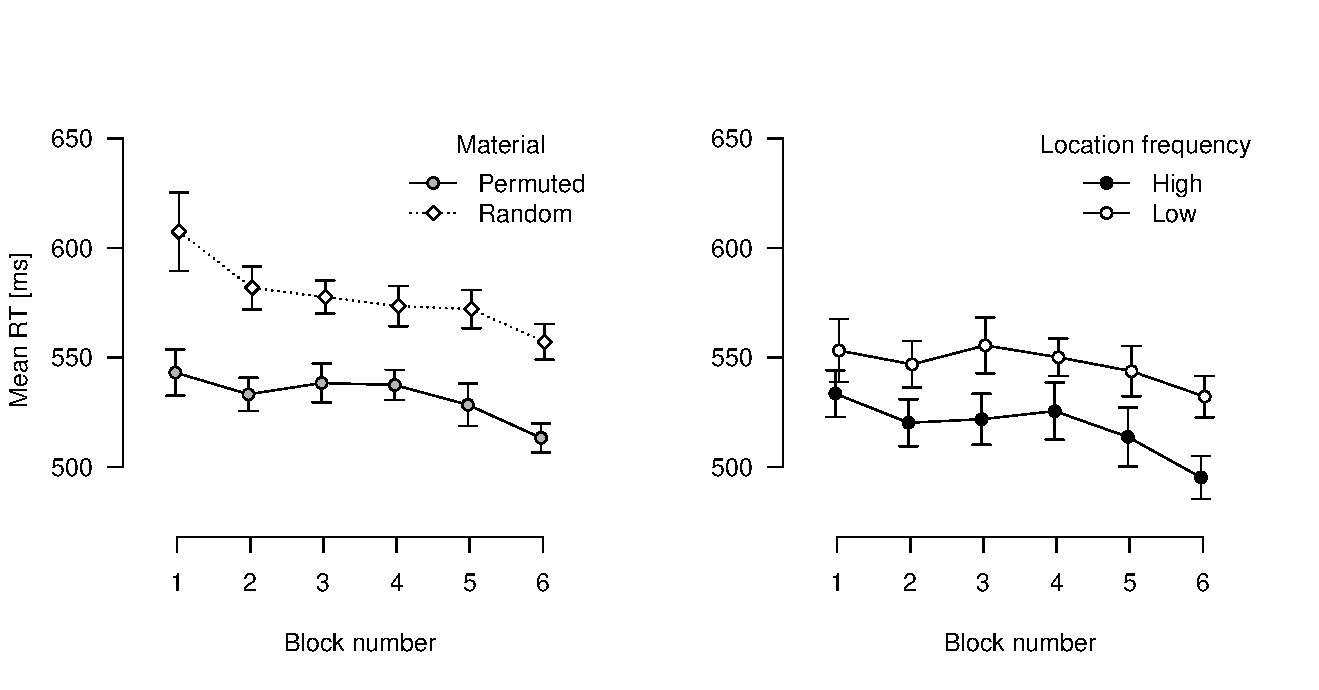
\includegraphics{manuscript_files/figure-latex/acquisition-rt-1.pdf}
\caption{\label{fig:acquisition-rt}Left: Mean reaction times for permuted (solid line) and random material (dashed line). Right: Mean reaction times for permuted material, split by high-frequency (filled circles) vs.~low-frequency locations (open circles). Error bars represent 95\% within-subjects CIs.}
\end{figure}

The mean RTs obtained over training blocks are shown in the left panel of Figure \ref{fig:acquisition-rt}, separately for permuted and random material (in this and all following training-phase analyses, we excluded RTs of the first trial of each block and of trials that resulted in an error).
Analysing RTs using a 2 (\emph{material}: permuted vs.~random) \(\times\) 6 (\emph{block number}) ANOVA revealed a significant main effect of \emph{material}, , with slower responses for random material than for permuted material, and a significant main effect of \emph{block number}, , reflecting practice effects.
The factors \emph{material} and \emph{block number} did not interact, , indicating that any knowledge was acquired already during the first block.

For the group with permuted material, some locations were presented twice within each pseudo-sequence.
The right panel of Figure \ref{fig:acquisition-rt} shows the mean RTs for these two types of stimuli. A 2 (\emph{frequency}: high vs.~low) \(\times\) 6 (\emph{block number}) ANOVA revealed a main effect of \emph{frequency}, ; high-frequency responses were faster than low-frequency responses.
The main effect of \emph{block number} was also significant, , but not the interaction, .
These findings suggest that participants in the \emph{permuted} condition acquired some form of simple response-location frequency knowledge that benefitted their SRTT performance, and especially so for the more frequent responses.

\hypertarget{generation-task}{%
\subsection{Generation task}\label{generation-task}}

In the free generation condition, after an initial sequence of three cue trials, participants freely generated 120 consecutive response locations.
In the cued generation condition, in each of 120 trials, three to five stimulus locations (taken from learning materials) were presented as cues and participants had to respond with the corresponding key.
For each of the 120 trials, a response \emph{triplet} consisted of the previous two locations as well as the location of the current response
(in the cued generation condition, the response triplet consisted of the last two cue locations and the current response location;
in the free generation condition, the response triplet consisted of the previous two response locations as well as the current response location;
for the first two trials of each generation block, the locations of the corresponding cue trials were used).
We calculated the proportion of triplets that were consistent with training sequences (see Appendix A).\footnote{Because we only used pseudo-random sequences in this study, we defined that, given the last two locations,
  the location that was most frequently presented after these two locations during training as being the ``correct'' response.
  For the \emph{no-learning} condition, correct responses were computed on the basis of sequences identical to those used in the \emph{random} group.}
Figure \ref{fig:generation-soc} depicts the pattern of correctly generated triplets as a function of generation task, material, and PD instruction.

\hypertarget{correctly-generated-second-order-transitions}{%
\subsubsection{Correctly generated second-order transitions}\label{correctly-generated-second-order-transitions}}



\begin{figure}
\centering
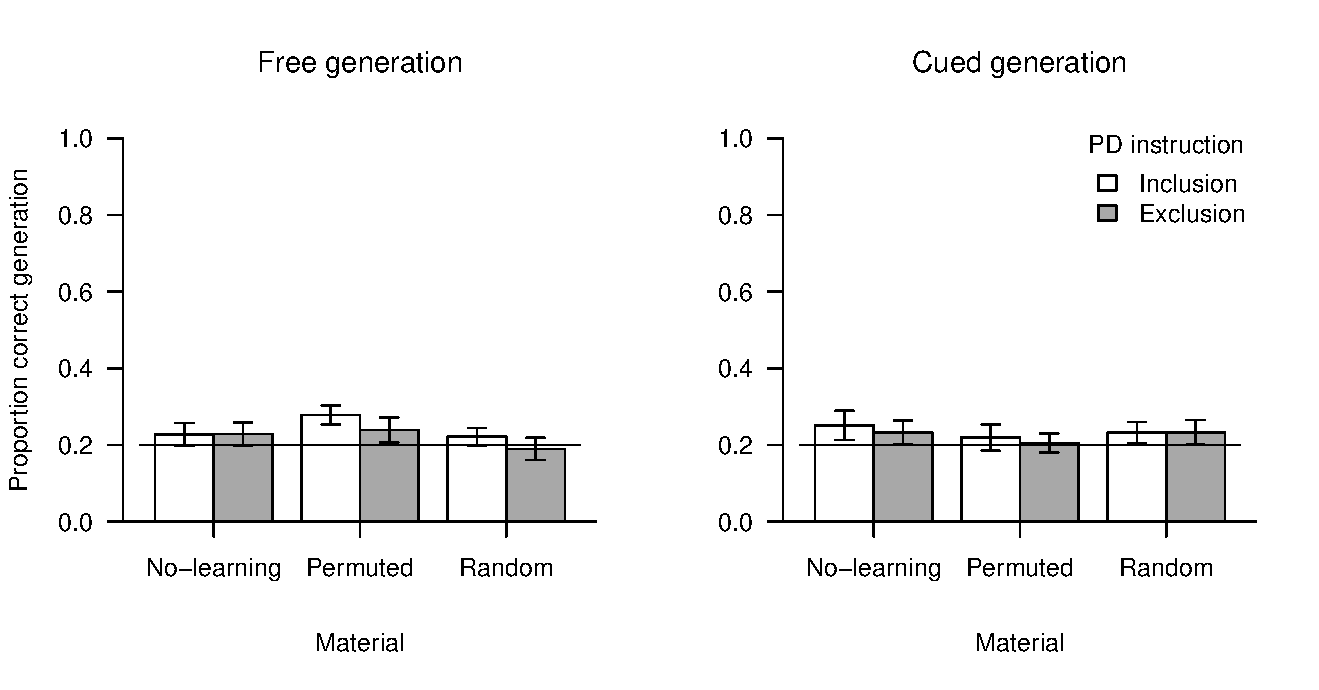
\includegraphics{manuscript_files/figure-latex/generation-soc-1.pdf}
\caption{\label{fig:generation-soc}Proportions of correctly generated triplets during PD generation task (chance level = .2). Error bars represent 95\% CIs.}
\end{figure}

The proportions of correctly generated triplets were analysed using a 3 (\emph{material}: permuted vs.~random vs.~no-learning) \(\times\) 2 (\emph{generation task}: free vs.~cued) \(\times\) 2 (\emph{PD instruction}: inclusion vs.~exclusion) \(\times\) 2 (\emph{order}: inclusion first vs.~exclusion first) ANOVA.
It revealed a main effect of \emph{PD instruction}, , more correct triplets were generated during inclusion than during exclusion blocks.
This \(I > E\) pattern suggests the presence of explicit knowledge, despite the absence of sequence information in the training material.

The ANOVA also revealed an interaction of \emph{material} \(\times\) \emph{generation task}, .
Analysing only free generation using a 3 (\emph{material}: permuted vs.~random vs.~no-learning) \(\times\) 2 (\emph{PD instruction}: inclusion vs.~exclusion) \(\times\) 2 (\emph{order}: inclusion first vs.~exclusion first) ANOVA revealed a main effect of \emph{material}, (and again the main effect of \emph{PD instruction}, ).
Tukey's HSDs revealed a significant difference between \emph{permuted} and \emph{random}, \(\Delta M = 0.05\), \(95\%\ \mathrm{CI}_\mathrm{\scriptsize Tukey(3)}\) \([0.02, 0.09]\), \(t(83) = 3.66\), \(p_\mathrm{\scriptsize Tukey(3)} = .001\), the difference between \emph{permuted} and \emph{no-learning} group trended to be significant, \(\Delta M = -0.03\), \(95\%\ \mathrm{CI}_\mathrm{\scriptsize Tukey(3)}\) \([-0.06, 0.00]\), \(t(83) = -2.17\), \(p_\mathrm{\scriptsize Tukey(3)} = .083\), \emph{random} and \emph{no-learning} groups did not differ from each other, \(\Delta M = 0.02\), \(95\%\ \mathrm{CI}_\mathrm{\scriptsize Tukey(3)}\) \([-0.01, 0.05]\), \(t(83) = 1.59\), \(p_\mathrm{\scriptsize Tukey(3)} = .257\).
Analysing only cued generation revealed no effects, suggesting that the free generation task was more sensitive in picking up learning effects on generation performance.

To summarize, there was a main effect of PD instruction as well as an effect of material in the free-generation data; no effects were obtained in the cued-generation data.
In the process-dissociation logic, the effect of PD instruction suggests the presence of explicit knowledge.
In addition, the effect of material suggests the presence of implicit knowledge in the permuted condition.
Next, we will apply two different PD analysis stategies to these data to investigate more formally whether, given the assumptions underlying the PD approach can be upheld, the pattern is indeed indicative of the presence of explicit and implicit knowledge.

\hypertarget{ordinal-pd}{%
\subsubsection{Ordinal PD}\label{ordinal-pd}}

{[}\ldots{]}

Comparing the \emph{permuted} and \emph{no-learning} conditions, performance was greater in the \emph{permuted} group under inclusion instructions but was identical in both groups under exclusion instructions.
This data pattern implies increased levels of both the automatic and the controlled process in the permuted as compared to the no-learning condition.
Comparing the \emph{permuted} and \emph{random} conditions, performance was greater in the \emph{permuted} group under both inclusion and exclusion instructions.
This data pattern implies an increase in the automatic process in the permuted as compared to the random condition but no effect on controlled process.

These results suggest that participants acquire some form of implicit knowledge from permuted material that they can use to produce above-chance levels of correct triplets in the free generation task. They also suggest that the permuted and random materials allow participants to acquire some form of explicit knowledge which they can use to perform better under inclusion than under exclusion conditions.

\hypertarget{pd-equations}{%
\subsubsection{PD equations}\label{pd-equations}}

{[}\ldots{]}

\hypertarget{interim-summary}{%
\subsection{Interim summary}\label{interim-summary}}

In three different control conditions, we computed the proportion of generated responses that matched the learning materials to test for any effect of implicit or explicit knowledge acquired from the learning phase.
We obtained converging evidence from three different approaches:
(1) In ANOVAs, the proportions of correctly generated responses differed as a function of material (this effect was restricted to the free generation task), as well as of PD instruction.
(2) The ordinal PD approach, when applied to the free generation data, yielded evidence for greater implicit knowledge in the permuted than in the random and no-learning groups.
It also yielded evidence for explicit knowledge in the permuted condition (and, by implication, in the random condition).
(3) The PD equations yielded estimates of the controlled process, reflecting explicit knowledge, that were significantly different from zero for the free-generation data.
They also yielded estimates of the automatic process, reflecting implicit knowledge, that were above chance levels for 4 out of 6 experimental conditions.

Taken together, despite the fact that the material in the learning phase did not contain any sequence information, the PD approach using generation tasks yielded `evidence' for both implicit and explicit knowledge.
In the following sections, we will try to account for these findings in terms of sequence-unrelated frequency properties, response tendencies, and cueing artifacts.

\hypertarget{sequence-unrelated-frequency-properties}{%
\subsection{Sequence-unrelated frequency properties}\label{sequence-unrelated-frequency-properties}}

{[}\ldots{]}

\hypertarget{effects-of-generation-task}{%
\subsection{Effects of generation task}\label{effects-of-generation-task}}

Whereas the proportion of reversals as well as high-frequency locations affected performance in free generation, similar influences were not observed on cued-generation data.
This suggests that the cued generation task may be less sensitive to subtle effects of learning.
The cued generation task has been criticized because the cues may contain information about the sequence that may affect generation performance and distort estimates of learning.
Here we investigated potential effects of cues on generation responses that may occur even in control conditions and in the absence of informational influence.

As cues, participants were presented with brief segments of response locations taken from the learning phase.
It is known that recent responses may be less likely to be generated (e.g., Boyer, Destrebecqz, \& Cleeremans, 2005).
This bias may affect generation performance selectively in the \emph{permuted} condition.
Because the permuted material contained high-frequency as well as low-frequency response locations, the same was true for the cues presented to participants in the permuted condition during the cued-generation task.
As a consequence, the bias to avoid recent locations would apply more strongly to high-frequency locations.
This could account for the above finding that high-frequency locations were generated at below-chance levels in the cued generation task, and for the suppressed levels of correct performance in the permuted condition in that task.



\begin{figure}
\centering
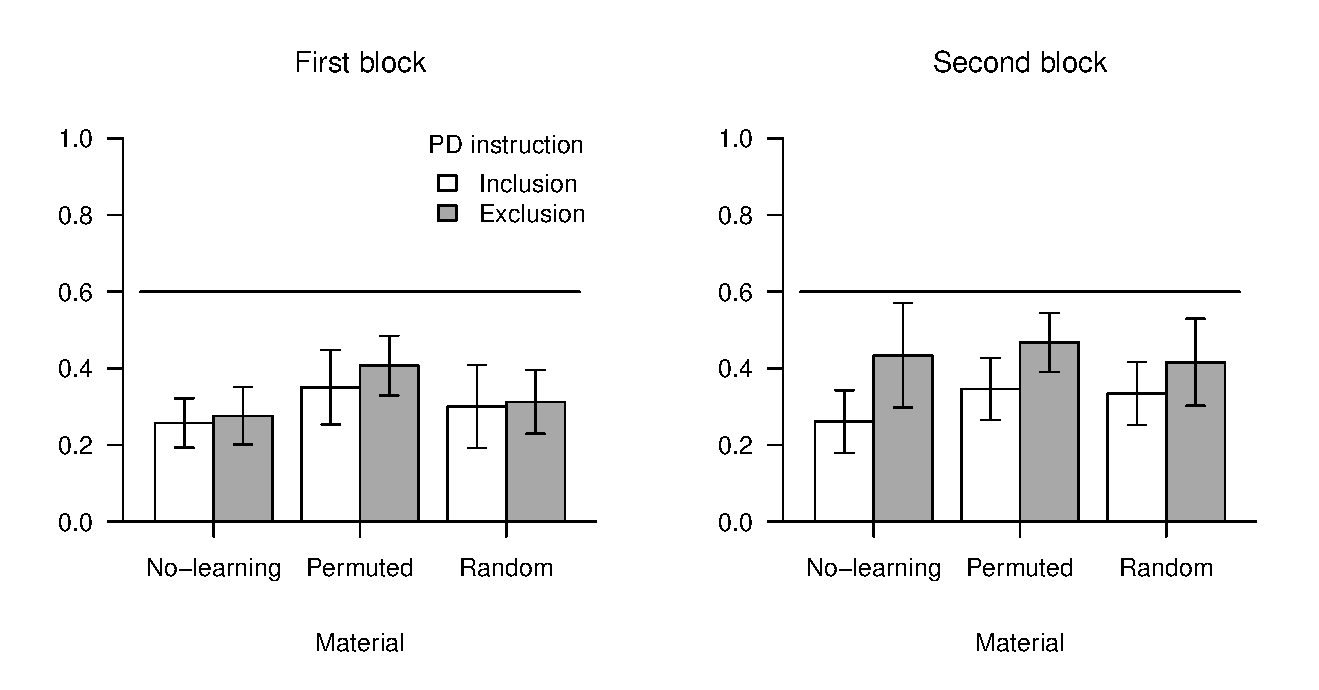
\includegraphics{manuscript_files/figure-latex/was-cue-including-reversals-1.pdf}
\caption{\label{fig:was-cue-including-reversals}Proportions of locations generated in the cued generation task that were presented as a cue on their respective trial, separately for the first and the second generation block (chance level = .6). Error bars represent 95\% CIs.}
\end{figure}

For the cued generation task, Figure \ref{fig:was-cue-including-reversals} shows the proportion of response locations that were also presented as a cue on their respective trial.
With three to five cues presented on each trial (and direct repetitions prohibited and excluded from analyses),
chance level of generating a location that had just been presented equalled \(3/5 = .6\).

A 3 (\emph{material}: permuted, random, no-learning) \(\times\) 2 (\emph{PD instruction}: inclusion vs.~exclusion) \(\times\) 2 (\emph{block order}: inclusion first vs.~exclusion first) ANOVA revealed a main effect of \emph{material}, .
Tukey's HSDs revealed a significant difference between the \emph{permuted} and \emph{no-learning} groups, \(\Delta M = -0.09\), \(95\%\ \mathrm{CI}_\mathrm{\scriptsize Tukey(3)}\) \([-0.16, -0.01]\), \(t(86) = -2.59\), \(p_\mathrm{\scriptsize Tukey(3)} = .030\), all other \emph{p}s \textgreater{} .24.
The ANOVA also revealed a main effect of \emph{PD instruction}, : more repetitions of cue locations were generated under exclusion conditions.
This effect was qualified by an interaction \emph{PD instruction} \(\times\) \emph{block order}, , which indicates that the effect of PD instruction differed between participants who worked under inclusion instructions in the first generation block and under exclusion instructions in the second block and those who received the PD instructions in the reverse order. To further explore this interaction, we analysed first and second blocks using separate ANOVAs, thus turning the \emph{PD instruction} factor into a between-subjects factor.
In the first block, only the main effect of \emph{material} turned out to be significant, .
In the second block, only the main effect of \emph{PD instruction} was significant, .

These results suggest three conclusions:
First, the fact that the tendency to avoid generating cued locations was also present in the no-learning condition suggests that it was not acquired during the SRTT training but either reflects pre-experimental response tendencies, or, alternatively, it may reflect a tendency of the cued generation task to bias generation performance against repeating the cue locations.

Second, the cue-avoidance bias was influenced by the type of learning material in the first but not the second block.
This suggests that, while the cued generation task is sensitive to effects of learning during the first block, this is no longer the case during the second block.
This finding further supports the notion that the cued generation format may affect generation performance, and that over time this influence becomes stronger than the effects of learning.

Third, cue-avoidance bias was stronger under inclusion than under exclusion instructions in the second block of the generation task.
This suggests that participants can acquire response strategies during the cued-generation task that help them produce different outcomes under inclusion and exclusion instructions.

Whether or not this tendency leads to artificially elevated levels of correct responses largely depends on the sequence material that is used.
Common sequences (e.g., Fu, Dienes, \& Fu, 2010; Fu, Fu, \& Dienes, 2008; Wilkinson \& Shanks, 2004) contain only one reversal within a four-position sequence consisting of 12 triplets.
Typically, only two locations are presented as cues on each trial to avoid informative influences, and direct repetitions are not allowed.
In this case, the strategy to avoid generating a cue location would lead to a correct-performance rate of approximately 46\% (i.e., a .5 chance to generate a correct response for 11 out of 12 triplets and a zero chance for the single reversal among the 12 triplets).
This is rather high relative to a chance-level baseline of .33 (c.f., Fu, Dienes, \& Fu, 2010).

To summarise, in the cued generation task, participants avoid generating a response that had been part of the cue sequence. This finding was independent of the type of training material, and it occurred even for the no-learning grooup, suggesting that it is a training-independent response tendency (i.e., a bias against generating locations present in the cue segment).

The findings further suggest that, in the permuted condition, this response strategy interacted with cue properties to influence generation performance.
Here, cue properties vary as a function of the frequency manipulation in the permuted condition:
Frequent locations are more likely to be included in the cue, and are therefore more likely to be subject to the avoidance bias;
this can explain the reduction, in the \emph{permuted} condition, of high-frequency responses in the cued as compared to the free generation task.

Finally, the cue-avoidance bias differed across PD instructions: cued responses were generated less frequently under inclusion than under exclusion instructions.
Interestingly, this difference emerged only in the second generation block, suggesting that the cued generation task allowed participants to acquire a strategy of selectively generating more cue locations under exclusion instructions:
If participants perceived the learning material as random, they will aim at generating a random sequence under inclusion instructions (i.e., generate a sequence similar to that in the learning phase);
under exclusion instructions, they will aim at generating a sequence that does not conform to their subjective notion of randomness (i.e., generate a sequence that is as dissimilar as possible to that in the learning phase).
When generating subjectively random sequences, participants typically produce more alternations and fewer repetitions than would be expected by chance (e.g., Boyer, Destrebecqz, \& Cleeremans, 2005).
By attempting to deviate from this subjectively experienced randomness they then generate more cue locations.

Taken together, the cued generation task was not only less sensitive to learning effects.
It also appears to induce -- or interact unfavorably with -- a bias to avoid recently generated response locations.
Both the below-chance generation of cue locations as well as its modulation by PD instruction may distort findings and conclusions regarding the presence or absence of explicit and implicit sequence knowledge.

\hypertarget{discussion}{%
\section{Discussion}\label{discussion}}

The present findings extend previous knowledge about the influence of pre-experimental response biases, simple frequency information, task format, and their interaction on performance in the generation task. First, it is known that zero-order frequency information may affect generation performance (Reed \& Johnson, 1994); here, we show that this effect depends on the type of generation task.
Second, it is known that, in cued generation, cues that carry information about the sequence may affect generation performance (Fu, Dienes, \& Fu, 2010).
We present first evidence that even in the absence of any sequence information, cues may affect generation performance by way of their simple frequency properties and in interaction with response tendencies.
Third, it is known that participants may be biased to avoid generating recent response locations (Boyer, Destrebecqz, \& Cleeremans, 2005).
Here, we demonstrated that this bias may interact with properties of the learning material (zero-order frequencies, proportion of reversals) and task format, and that it can differentially affect inclusion and exclusion performance.
These findings have important implications for the validity of the process-dissociation procedure as applied to the generation task.

\hypertarget{process-dissociation-results}{%
\subsection{Process-dissociation results}\label{process-dissociation-results}}

The present study realized three different control conditions, using different types of pseudo-random materials, in which participants could not learn any second-order regularity.
Implicit and explicit knowledge was assessed with the PD procedure, using two different generation tasks.
Despite the irregular learning materials, and independent of the type of analysis, the results of a comparison between performance in the permuted and random conditions in the free-generation task suggested the presence of implicit knowledge.
Similarly, independent of the type of analysis, the results also suggested the presence of explicit knowledge under some conditions (i.e., due to the asymmetric generation of reversals under inclusion versus exclusion instructions).
Finally, the results erroneously underestimated knowledge in some conditions: Although participants learned to distinguish between high- and low-frequency locations, they expressed this knowledge in the free-generation condition but did not express this knowledge in the cued-generation condition.
These findings illustrate that unwanted influences can affect generation performance and may thereby artificially inflate or mask estimates of implicit and explicit knowledge.

Taken together, the findings suggest that there are several problems with the PD approach in its application to investigating the processes underlying sequence learning when effects of extra-experimental influences on performance cannot be excluded.
In those cases, baseline performance may differ in inclusion and exclusion instructions and/or across experimental conditions.
Under those circumstances, the ordinal PD approach is no longer valid (Hirshman, 2004).\footnote{The ordinal PD approach assumes that baseline performance does not differ across conditions or tasks (see Hirshman, 2004, p.559, section ``Comparison of the Current Approach and the Process-Dissociation Procedure'' and Footnote 8). Such baseline differences may arise from different guessing or response bias, and they invalidate the conclusions that can be drawn from the comparison of performance in conditions. This is because the performance differences between conditions or tasks that are used to draw conclusions about differences in automatic and/or controlled processes may instead reflect baseline differences due to guessing or response bias.}
In other words, given the possible influence of response tendencies and their interaction with properties of the material, we cannot draw conclusions about the relative contribution of implicit and explicit knowledge by simply comparing inclusion and exclusion performance, be it directly (e.g., \(I > E\)), across experimental conditions (e.g., \(E_A > E_B\)), or with a baseline (e.g., \(E > B\)).
Instead, it is necessary to quantify the unwanted extraneous influence and separate it from the experimental effects of interest.
This can be done by extending the basic PD design and model.

\hypertarget{an-extended-pd-model}{%
\subsection{An extended PD model}\label{an-extended-pd-model}}

In applications of the PD, exclusion performance is sometimes compared to an a-priori chance level baseline.
The present study has shown that the proportion of correctly generated triplets may deviate from such an a-priori chance-level baseline, and may even differ across inclusion and exclusion conditions, in the absence of both implicit and explicit sequence knowledge.
In other words, we found that response tendencies, alone or in interaction with properties of the learning material, may affect generation performance, may cause deviations from a-priori chance baselines, and may distort the PD model's estimates of implicit and explicit knowledge.

To accommodate this potential confound, first, it is necessary to use an empirical baseline.
One could extend the PD design and model, as applied to the generation task, by adding a control condition along with separate response-tendency or nuisance parameters, as has been done by Buchner and colleagues for the recollection task (Buchner, Steffens, Erdfelder, \& Rothkegel, 1997; Buchner, Steffens, \& Rothkegel, 1998).
In the control condition, that is, in the absence of sequence knowledge, generation performance will then reflect sequence-unspecific properties of the material as well as response tendencies.
In the experimental condition, these same influences may affect generation performance over and above the effects of learning higher-order sequence information.
The nuisance parameter can then be equated across the control and experimental conditions, capture the unwanted influences, and separate them from the effects of implicit and explicit knowledge.
In this model, any differences in performance between the control and experimental conditions will be reflected in estimates of implicit and/or explicit knowledge.
Second, the problem that response tendencies may differentially affect inclusion and exclusion performance can be solved by using as separate baselines the performance of a control group in the inclusion and exclusion conditions, and by introducing one nuisance parameter for each condition.
Such an extended model allows for the possibility that response tendencies affect generation performance over and above explicit and implicit knowledge.
Similar extensions for capturing extraneous influences have been proposed and demonstrated as necessary and useful in other domains to address similar response-tendency issues {[}e.g., pre-experimental familiarity, Buchner, Erdfelder, and Vaterrodt-Plünnecke (1995); right-hand bias; Stahl and Degner (2007){]}.

The extended model's equations deviate from the original equations (see introduction) by including nuisance parameters that account for baseline performance (along the lines suggested by Buchner, Erdfelder, \& Vaterrodt-Plünnecke, 1995; Buchner, Steffens, Erdfelder, \& Rothkegel, 1997).
Because baseline performance may be different under inclusion and exclusion instructions, two different parameters \(R_{\mathrm{Inclusion}}\) and \(R_{\mathrm{Exclusion}}\) are added to the model.
The equations of the experimental conditions of the extended model are:
\(I_\mathrm{Experimental} = C + (1-C) \cdot A + (1-C) \cdot (1-A) \cdot R_{\mathrm{Inclusion}}\),
and
\(E_\mathrm{Experimental} = (1-C)A + (1-C)(1-A)R_{\mathrm{Exclusion}}\).
For the empirical control or baseline condition, it would be assumed that only extra-experimental or nuisance factors affect generation performance:
\(I_\mathrm{Control} = R_{\mathrm{Inclusion}}\),
and
\(E_\mathrm{Control} = R_{\mathrm{Exclusion}}\).

To illustrate, we applied this model to the permuted and random conditions in the free generation task.
Recall that both traditional approaches suggested the presence of explicit and implicit knowledge in the permuted group, as well as the presence of explicit knowledge in the random group.
The extended model allows us to quantify the effect of training with permuted material over a training phase with random material on controlled and automatic processes.
We used the random group as the empirical control condition; this is equivalent to the assumption that whatever affects performance in the random group can be subsumed as nuisance factors.
Estimates of \(R_{\mathrm{Inclusion}}\) and \(R_{\mathrm{Exclusion}}\) therefore reflect generation performance in the random group, \(R_{\mathrm{Inclusion}} = .251\) and \(R_{\mathrm{Exclusion}} = .228\).
Differences between the random and permuted condition are then reflected in the parameters for controlled and automatic processes.
Results of the extended model suggests that training with permuted material affected the automatic process, \(A = .047\), \(\Delta G^2_{(df=1)} = 16.44\), \(p < .001\), but did not affect the controlled process, \(C = .001\), \(\Delta G^2_{(df=1)} = 0.004\), \(p=.95\).
The effect on the automatic process -- implicit knowledge -- reflects the location frequency effect, and it is consistent with the finding that participants responded faster to high-frequency than to low-frequency locations during SRTT training.
The extended model indicates the absence of an effect on explicit knowledge.
The nuisance parameters capture the difference between inclusion and exclusion performance in both the random and permuted group that was interpreted as evidence for explicit knowledge in both the ordinal PD approach as well as in the original model equations.

Note that the levels of generation performance in the control condition can serve as valid baselines -- and the controlled and automatic parameters can be valid estimates -- only to the degree that the processes captured by the nuisance parameters are independent from explicit and implicit knowledge processes.
In other words, the extended model requires additional assumptions, namely that the processes underlying the parameters \(C\) and \(A\) are independent from the nuisance processes (e.g., guessing, response bias) that are reflected in the new parameters \(R_{\mathrm{Inclusion}}\) and \(R_{\mathrm{Exclusion}}\).
These assumptions are as of yet untested, and future research is needed to supply empirical evidence as to whether these new independence assumptions are met.

\hypertarget{free-versus-cued-generation}{%
\subsection{Free versus cued generation}\label{free-versus-cued-generation}}

In free generation, participants sometimes produce relatively sparse data, for instance, by repeatedly generating a small subset of all possible transitions, thereby generating missing data for the remaining transitions.
With the cued generation task, researchers can control the cues and thereby ensure that comparable (or at least considerable) numbers of observations are obtained for each transition.
This is an advantage especially when different types of transitions and their properties are to be compared in a within-subject approach.

However, the present findings support previous warnings that the cued generation task must be treated with caution because the choice of cues may influence generation performance (Fu, Dienes, \& Fu, 2010; Jiménez \& Vázquez, 2005).
In addition to previous findings regarding informative cues, the present study provides an additional argument against the cued generation task:
The tendency to avoid generating locations that were presented as cues may systematically bias generation performance, and may erroneously suggest the presence of both implicit and explicit knowledge.

In light of these problems, we currently do not see an empirical way of obtaining an equal number of observations for each transition in the generation task.
This could imply that attempts of modeling individual transitions as a within-participant factor will face additional challenges.
One way of avoiding artifacts resulting from a limited and biased selection of generated transitions is to use adequate weighting procedures.
For instance, researchers could compute correct-generation rates for each of the cells in the transition matrix and estimate participants' mean proportion of correctly generated transitions as a weighted average.

\hypertarget{limitations-and-open-questions}{%
\subsection{Limitations and open questions}\label{limitations-and-open-questions}}

We briefly sketch open research questions posed by the additional independence assumptions, discuss the current development of hierarchical multinomial modeling techniques, and note the potential influence of additional unknown factors affecting performance in the generation task.

\hypertarget{on-the-independence-assumptions-underlying-the-extended-model}{%
\subsubsection{On the independence assumptions underlying the extended model}\label{on-the-independence-assumptions-underlying-the-extended-model}}

As mentioned above, the extended PD model assumes that response tendencies as modelled by \(R_{\mathrm{Inclusion}}\) and \(R_{\mathrm{Exclusion}}\) are independent of controlled and automatic processes.
If this assumption is violated, parameter estimates are no longer valid measures of the underlying psychological processes.
This possiblity deserves to be taken seriously; in other domains, empirical violations of independence between controlled and automatic processes have been obtained (e.g., Rouder, Lu, Morey, Sun, \& Speckman, 2008).
The open question is whether response tendencies can be affected by the same properties of the learning material that may also affect implicit and explicit learning.
There are some findings in the literature that at least suggest such an interaction may well be possible.
For instance, participants tended to show lag effects (reflecting negative recency) in a permuted condition but not in a random condition (Boyer, Destrebecqz, \& Cleeremans, 2005).
Here, the tendency to avoid generating recent locations interacted with properties of the learning material.
Perhaps more critically, the present results suggest that in the permuted condition, the bias against generating cued locations was reduced whereas implicit knowledge was enhanced (i.e., participants learned about the frequency with which certain response locations occurred during training).
If the response bias is reduced in a condition with greater implicit knowledge, then the response bias estimates (i.e., the \(R\) parameters) obtained from the control condition (where implicit knowledge is lower or entirely absent) will tend to overestimate the response bias in that condition.
The present finding may reflect effects of other factors, but if such an interaction pattern between response tendency and implicit knowledge can be substantiated, it would constitute evidence against the independence assumption.
In turn, this would require further elaborating and refining the extended PD paradigm and model.

\hypertarget{data-aggregation-and-hierarchical-modeling}{%
\subsubsection{Data aggregation and hierarchical modeling}\label{data-aggregation-and-hierarchical-modeling}}

In our application of the PD model, we aggregated the data across participants, as this has been the standard procedure in common applications of PD and our aim was to illustrate potential problems with such applications.
Our results demonstrate that the PD procedure, as commonly applied, yields erroneous conclusions supporting the presence of implicit and/or explicit knowledge, even in the absence of such knowledge.
Note that such erroneous conclusions about the presence of an influence on parameters are less likely when, instead of aggregating, individual data are analyzed using hierarchical models.
This is because data aggregation assumes parameter homogeneity across participants, which is likely to be violated in most cases.
As a consequence of aggregation in the presence of heterogeneity, confidence intervals can be underestimated, and nominal statistical error levels can be violated by statistical tests.\footnote{We applied the hierarchical Bayesian PD model proposed by Rouder, Lu, Morey, Sun, and Speckman (2008) to the present data in order to account for person and item variability.
  The resulting parameter estimates are available in the supplemental material that can be obtained from \url{https://github.com/methexp/pdl1}.
  The results corroborated the findings obtained with the traditional analyses reported above (i.e., \(C>0\), \(A>.2\), and the ordering of \(A\) estimates across conditions).}

This problem does not arise if hierarchical modeling techniques are used (Klauer, 2006, 2010; e.g., Rouder, Lu, Morey, Sun, \& Speckman, 2008) that account for the heterogeneity across participants (and items) in their estimates of the parameters' variability.
Hierarchical models often draw a more realistic picture of the variability of parameter estimates.
In all cases in which parameters must be assumed to vary across participants, they should be preferred to the traditional approach of data aggregation.\footnote{The use and adoption of hierarchical modeling approaches is currently limited by the availability of general-purpose software (but see, e.g., Matzke, Dolan, Batchelder, \& Wagenmakers, 2013; Stahl \& Klauer, 2007).}

\hypertarget{characteristics-of-response-tendencies}{%
\subsubsection{Characteristics of response tendencies}\label{characteristics-of-response-tendencies}}

In the present study, we obtained evidence that participants may use two types of response tendencies:
First, they generated fewer reversals than expected by chance.
Second, in the cued generation task, they avoided generating responses that were part of the cue segments.
It is unclear whether these patterns reflect the same bias (e.g., based on subjective notions of randomness) or whether they reflect different response tendencies, and whether they reflect consciously applied strategies or rather more implicit trends.
In addition, results obtained with the extended model suggested that, even in the absence of both implicit and explicit knowledge and after controlling for the identified response tendencies, there are other unknown factors that allow participants to perform better than chance, and even better under inclusion than under exclusion conditions.
Future research should address these questions in order to better understand their potential for affecting generation performance.

\hypertarget{conclusion}{%
\subsection{Conclusion}\label{conclusion}}

Broadly speaking, the process-dissociation approach is to create two (or more) experimental conditions within a given experimental paradigm so that there is overlap with regard to most but not all of the psychological processes that are relevant for performance.
Combined with measurement models such as the PD equations or more complex multinomial models, this general approach has been extremely valuable and has been fruitful in a wide variety of research areas and experimental paradigms (Erdfelder et al., 2009; Yonelinas \& Jacoby, 2012).
Whereas a simple and elegant design is generally preferable, the present findings suggest that the application of process-dissociation methodology to the generation task may require more differentiation of experimental design and measurement model.

\newpage

\hypertarget{references}{%
\section{References}\label{references}}

\begingroup
\setlength{\parindent}{-0.5in}
\setlength{\leftskip}{0.5in}

\hypertarget{refs}{}
\begin{CSLReferences}{1}{0}
\leavevmode\hypertarget{ref-boyer_processing_2005}{}%
Boyer, M., Destrebecqz, A., \& Cleeremans, A. (2005). Processing abstract sequence structure: Learning without knowing, or knowing without learning? \emph{Psychological Research}, \emph{69}(5-6), 383--398. \url{https://doi.org/10.1007/s00426-004-0207-4}

\leavevmode\hypertarget{ref-buchner_unbiased_1995}{}%
Buchner, A., Erdfelder, E., \& Vaterrodt-Plünnecke, B. (1995). Toward {Unbiased Measurement} of {Conscious} and {Unconscious Memory Processes} within the {Process Dissociation Framework}. \emph{Journal of Experimental Psychology: General}, \emph{124}(2), 137--160. \url{https://doi.org/10.1037/0096-3445.124.2.137}

\leavevmode\hypertarget{ref-buchner_multinomial_1997}{}%
Buchner, A., Steffens, M. C., Erdfelder, E., \& Rothkegel, R. (1997). A multinomial model to assess fluency and recollection in a sequence learning task. \emph{The Quarterly Journal of Experimental Psychology A: Human Experimental Psychology}, \emph{50A}(3), 631--663. \url{https://doi.org/10.1080/027249897392053}

\leavevmode\hypertarget{ref-buchner_role_1998}{}%
Buchner, A., Steffens, M. C., \& Rothkegel, R. (1998). On the {Role} of {Fragmentary Knowledge} in a {Sequence Learning Task}. \emph{The Quarterly Journal of Experimental Psychology Section A}, \emph{51}(2), 251--281. \url{https://doi.org/10.1080/713755757}

\leavevmode\hypertarget{ref-curran_violations_1995}{}%
Curran, T., \& Hintzman, D. L. (1995). Violations of the {Independence Assumption} in {Process Dissociation}. \emph{Journal of Experimental Psychology: Learning, Memory, and Cognition}, \emph{21}(3), 531--547. \url{https://doi.org/10.1037/0278-7393.21.3.531}

\leavevmode\hypertarget{ref-destrebecqz_can_2001}{}%
Destrebecqz, A., \& Cleeremans, A. (2001). Can {Sequence Learning Be Implicit}? {New Evidence} with the {Process Dissociation Procedure}. \emph{Psychonomic Bulletin \& Review}, \emph{8}(2), 343--350. \url{https://doi.org/10.3758/BF03196171}

\leavevmode\hypertarget{ref-dienes_gambling_2010}{}%
Dienes, Z., \& Seth, A. (2010). Gambling on the {Unconscious}: {A Comparison} of {Wagering} and {Confidence Ratings} as {Measures} of {Awareness} in an {Artificial Grammar Task}. \emph{Consciousness and Cognition}, \emph{19}(2), 674--681. \url{https://doi.org/10.1016/j.concog.2009.09.009}

\leavevmode\hypertarget{ref-erdfelder_multinomial_2009}{}%
Erdfelder, E., Auer, T.-S., Hilbig, B. E., Aßfalg, A., Moshagen, M., \& Nadarevic, L. (2009). Multinomial {Processing Tree Models}: {A} review of the literature. \emph{Zeitschrift für Psychologie / Journal of Psychology}, \emph{217}(3), 108--124. \url{https://doi.org/10.1027/0044-3409.217.3.108}

\leavevmode\hypertarget{ref-fu_can_2010}{}%
Fu, Q., Dienes, Z., \& Fu, X. (2010). Can {Unconscious Knowledge Allow Control} in {Sequence Learning}? \emph{Consciousness and Cognition}, \emph{19}(1), 462--474. \url{https://doi.org/10.1016/j.concog.2009.10.001}

\leavevmode\hypertarget{ref-fu_implicit_2008}{}%
Fu, Q., Fu, X., \& Dienes, Z. (2008). Implicit {Sequence Learning} and {Conscious Awareness}. \emph{Consciousness and Cognition}, \emph{17}(1), 185--202. \url{https://doi.org/10.1016/j.concog.2007.01.007}

\leavevmode\hypertarget{ref-haider_old_2011}{}%
Haider, H., Eichler, A., \& Lange, T. (2011). An {Old Problem}: {How Can We Distinguish} between {Conscious} and {Unconscious Knowledge Acquired} in an {Implicit Learning Task}? \emph{Consciousness and Cognition}, \emph{20}(3), 658--672. \url{https://doi.org/10.1016/j.concog.2010.10.021}

\leavevmode\hypertarget{ref-hirshman_logic_1998}{}%
Hirshman, E. (1998). On the {Logic} of {Testing} the {Independence Assumption} in the {Process}-{Dissociation Procedure}. \emph{Memory \& Cognition}, \emph{26}(5), 857--859. \url{https://doi.org/10.3758/BF03201168}

\leavevmode\hypertarget{ref-hirshman_ordinal_2004}{}%
Hirshman, E. (2004). Ordinal {Process Dissociation} and the {Measurement} of {Automatic} and {Controlled Processes}. \emph{Psychological Review}, \emph{111}(2), 553--560. \url{https://doi.org/10.1037/0033-295X.111.2.553}

\leavevmode\hypertarget{ref-jacoby_process_1991}{}%
Jacoby, L. L. (1991). A {Process Dissociation Framework}: {Separating Automatic} from {Intentional Uses} of {Memory}. \emph{Journal of Memory and Language}, \emph{30}(5), 513--541. \url{https://doi.org/10.1016/0749-596X(91)90025-F}

\leavevmode\hypertarget{ref-jimenez_sequence_2005}{}%
Jiménez, L., \& Vázquez, G. A. (2005). Sequence {Learning} under {Dual}-{Task Conditions}: {Alternatives} to a {Resource}-{Based Account}. \emph{Psychological Research}, \emph{69}(5-6), 352--368. \url{https://doi.org/10.1007/s00426-004-0210-9}

\leavevmode\hypertarget{ref-klauer_hierarchical_2006}{}%
Klauer, K. C. (2006). Hierarchical {Multinomial Processing Tree Models}: {A Latent}-{Class Approach}. \emph{Psychometrika}, \emph{71}(1), 7--31. \url{https://doi.org/10.1007/s11336-004-1188-3}

\leavevmode\hypertarget{ref-klauer_hierarchical_2010}{}%
Klauer, K. C. (2010). Hierarchical {Multinomial Processing Tree Models}: {A Latent}-{Trait Approach}. \emph{Psychometrika}, \emph{75}(1), 70--98. \url{https://doi.org/10.1007/s11336-009-9141-0}

\leavevmode\hypertarget{ref-klauer_invariance_2015}{}%
Klauer, K. C., Dittrich, K., Scholtes, C., \& Voss, A. (2015). The {Invariance Assumption} in {Process}-{Dissociation Models}: {An Evaluation Across Three Domains}. \emph{Journal of Experimental Psychology: General}, \emph{144}(1), 198--221. \url{https://doi.org/10.1037/xge0000044}

\leavevmode\hypertarget{ref-matzke_bayesian_2013}{}%
Matzke, D., Dolan, C. V., Batchelder, W. H., \& Wagenmakers, E.-J. (2013). Bayesian {Estimation} of {Multinomial Processing Tree Models} with {Heterogeneity} in {Participants} and {Items}. \emph{Psychometrika}, \emph{80}(1), 205--235. \url{https://doi.org/10.1007/s11336-013-9374-9}

\leavevmode\hypertarget{ref-norman_fringe_2006}{}%
Norman, E., Price, M. C., \& Duff, S. C. (2006). Fringe consciousness in sequence learning: {The} influence of individual differences. \emph{Consciousness and Cognition}, \emph{15}(4), 723--760. \url{https://doi.org/10.1016/j.concog.2005.06.003}

\leavevmode\hypertarget{ref-persaud_postdecision_2007}{}%
Persaud, N., McLeod, P., \& Cowey, A. (2007). Post-{Decision Wagering Objectively Measures Awareness}. \emph{Nature Neuroscience}, \emph{10}(2), 257--261. \url{https://doi.org/10.1038/nn1840}

\leavevmode\hypertarget{ref-R-base}{}%
R Core Team. (2021). \emph{R: A language and environment for statistical computing}. Vienna, Austria: R Foundation for Statistical Computing. Retrieved from \url{https://www.R-project.org/}

\leavevmode\hypertarget{ref-reed_assessing_1994}{}%
Reed, J., \& Johnson, P. (1994). Assessing {Implicit Learning} with {Indirect Tests}: {Determining What Is Learned} about {Sequence Structure}. \emph{Journal of Experimental Psychology: Learning, Memory, and Cognition}, \emph{20}(3), 585--594. \url{https://doi.org/10.1037/0278-7393.20.3.585}

\leavevmode\hypertarget{ref-rouder_hierarchical_2008}{}%
Rouder, J. N., Lu, J., Morey, R. D., Sun, D., \& Speckman, P. L. (2008). A {Hierarchical Process}-{Dissociation Model}. \emph{Journal of Experimental Psychology: General}, \emph{137}(2), 370--389. \url{https://doi.org/10.1037/0096-3445.137.2.370}

\leavevmode\hypertarget{ref-stadler_statistical_1992}{}%
Stadler, M. A. (1992). Statistical {Structure} and {Implicit Serial Learning}. \emph{Journal of Experimental Psychology: Learning, Memory, and Cognition}, \emph{18}(2), 318--327. \url{https://doi.org/10.1037/0278-7393.18.2.318}

\leavevmode\hypertarget{ref-stahl_assessing_2007}{}%
Stahl, C., \& Degner, J. (2007). Assessing {Automatic Activation} of {Valence}: {A Multinomial Model} of {EAST Performance}. \emph{Experimental Psychology}, \emph{54}(2), 99--112. \url{https://doi.org/10.1027/1618-3169.54.2.99}

\leavevmode\hypertarget{ref-stahl_hmmtree_2007}{}%
Stahl, C., \& Klauer, K. C. (2007). {HMMTree}: {A Computer Program} for {Latent}-{Class Hierarchical Multinomial Processing Tree Models}. \emph{Behavior Research Methods}, \emph{39}(2), 267--273. \url{https://doi.org/10.3758/BF03193157}

\leavevmode\hypertarget{ref-wilkinson_intentional_2004}{}%
Wilkinson, L., \& Shanks, D. R. (2004). Intentional {Control} and {Implicit Sequence Learning}. \emph{Journal of Experimental Psychology: Learning, Memory, and Cognition}, \emph{30}(2), 354--369. \url{https://doi.org/10.1037/0278-7393.30.2.354}

\leavevmode\hypertarget{ref-yonelinas_processdissociation_2012}{}%
Yonelinas, A. P., \& Jacoby, L. L. (2012). The {Process}-{Dissociation Approach Two Decades Later}: {Convergence}, {Boundary Conditions}, and {New Directions}. \emph{Memory \& Cognition}, \emph{40}(5), 663--680. \url{https://doi.org/10.3758/s13421-012-0205-5}

\end{CSLReferences}

\endgroup


\clearpage
\makeatletter
\efloat@restorefloats
\makeatother


\begin{appendix}
\section{}



\begin{table}[h]

\begin{center}
\begin{threeparttable}

\caption{\label{tab:unnamed-chunk-2}Means (\(M\)) and standard errors (\(\mathit{SE}\))
of proportion of correctly generated second-order conditionals (SOCs).}

\begin{tabular}{lllllll}
\toprule
&  &  & \multicolumn{2}{c}{Inclusion} & \multicolumn{2}{c}{Exclusion} \\
\cmidrule(r){4-5} \cmidrule(r){6-7}
Material & \multicolumn{1}{c}{Generation task} & \multicolumn{1}{c}{Order} & \multicolumn{1}{c}{$M$} & \multicolumn{1}{c}{$\mathit{SE}$} & \multicolumn{1}{c}{$M$} & \multicolumn{1}{c}{$\mathit{SE}$}\\
\midrule
No learning & Cued & Exclusion first & .28 & .03 & .24 & .02\\
&  & Inclusion first & .22 & .02 & .22 & .03\\
& Free & Exclusion first & .22 & .02 & .24 & .02\\
&  & Inclusion first & .24 & .02 & .21 & .02\\ \midrule
Permuted & Cued & Exclusion first & .19 & .03 & .20 & .02\\
&  & Inclusion first & .24 & .02 & .21 & .02\\
& Free & Exclusion first & .27 & .02 & .25 & .02\\
&  & Inclusion first & .29 & .01 & .23 & .02\\ \midrule
Random & Cued & Exclusion first & .23 & .01 & .23 & .02\\
&  & Inclusion first & .23 & .02 & .24 & .03\\
& Free & Exclusion first & .21 & .02 & .18 & .01\\
&  & Inclusion first & .23 & .01 & .20 & .02\\ \midrule
\bottomrule
\end{tabular}

\end{threeparttable}
\end{center}

\end{table}
\end{appendix}

\end{document}
